\chapter{Double Scenario Classification of the last shared app, KFold Validation}Starting with fitting randomly the classifiers, there are some statistics of the data used for the first test: \\
 {\def\arraystretch{1.3} 
 \begin{table}[H] 
\centering 
\begin{tabular}{|l|l|l|} 
\hline 
  &count train  &count test  \\ \hline
messenger  &302  &748  \\ \hline
telegram  &314  &736  \\ \hline
whatsapp  &340  &710  \\ \hline
original  &94  &256  \\ \hline
\end{tabular} 
\end{table} }
\section{Logistic regression results:} 
Confusion matrix with number of sample and with normalization:
 {\def\arraystretch{1.3} 
 \begin{table}[H] 
\centering 
\begin{tabular}{|l|l|l|l|l|} 
\hline 
  &messenger  &telegram  &whatsapp  &original  \\ \hline
messenger  &746  &0  &2  &0  \\ \hline
telegram  &0  &618  &118  &0  \\ \hline
whatsapp  &0  &216  &494  &0  \\ \hline
original  &0  &0  &8  &248  \\ \hline
\end{tabular} 
\end{table} }

 \begin{figure}[H] 
\centering 
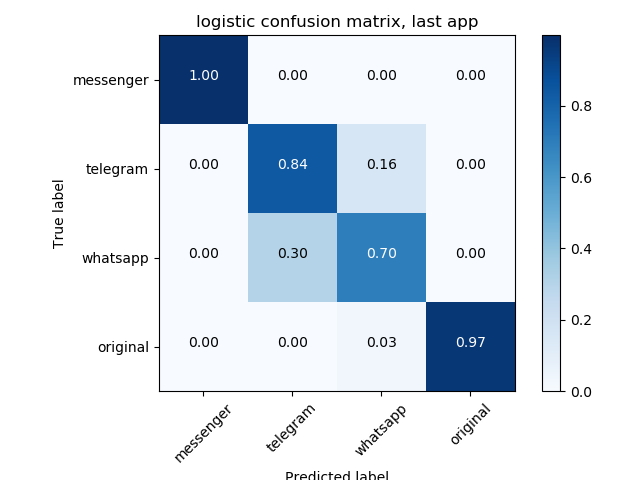
\includegraphics[scale=.6]{images/new_met_lr_initial_double_simple.png} 
\caption{logistic regression, last app classified} 
\end{figure} 


Result of the KFold validation with 10 bins:
 {\def\arraystretch{1.3} 
 \begin{table}[H] 
\centering 
\begin{tabular}{|l |l |l |l |l |l |l |l |l |l |}  
\hline 
0.8476&
0.8000&
0.9143&
0.8667&
0.8286&
0.8762&
0.8381&
0.8190&
0.8476&
0.8571\\ \hline  

\end{tabular} 
\end{table} }

The mean is : 0.849524\section{Linear Support Vector Machine results:} 
Confusion matrix with number of sample and with normalization:
 {\def\arraystretch{1.3} 
 \begin{table}[H] 
\centering 
\begin{tabular}{|l|l|l|l|l|} 
\hline 
  &messenger  &telegram  &whatsapp  &original  \\ \hline
messenger  &730  &6  &12  &0  \\ \hline
telegram  &0  &535  &201  &0  \\ \hline
whatsapp  &1  &197  &511  &1  \\ \hline
original  &0  &0  &6  &250  \\ \hline
\end{tabular} 
\end{table} }

 \begin{figure}[H] 
\centering 
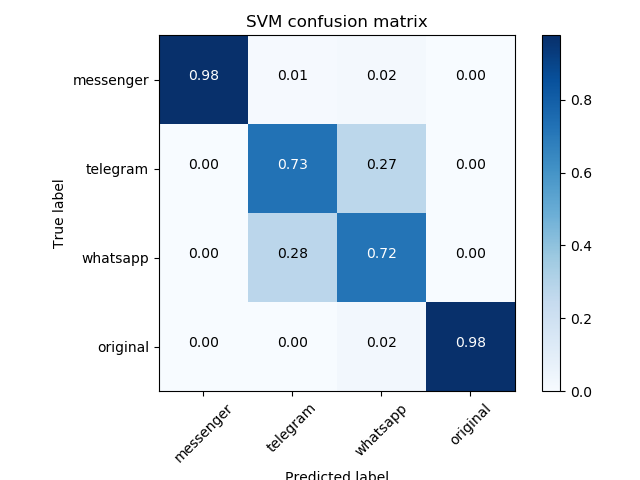
\includegraphics[scale=.6]{images/new_met_lsvm_initial_double_simple.png} 
\caption{linear SVM, last app classified} 
\end{figure} 


Result of the KFold validation with 10 bins:
 {\def\arraystretch{1.3} 
 \begin{table}[H] 
\centering 
\begin{tabular}{|l |l |l |l |l |l |l |l |l |l |}  
\hline 
0.8476&
0.8095&
0.8667&
0.7905&
0.7810&
0.8857&
0.8000&
0.8000&
0.8000&
0.8571\\ \hline  

\end{tabular} 
\end{table} }

The mean is : 0.823810\section{Random forest results:} 
Confusion matrix with number of sample and with normalization:
 {\def\arraystretch{1.3} 
 \begin{table}[H] 
\centering 
\begin{tabular}{|l|l|l|l|l|} 
\hline 
  &messenger  &telegram  &whatsapp  &original  \\ \hline
messenger  &740  &0  &8  &0  \\ \hline
telegram  &0  &627  &109  &0  \\ \hline
whatsapp  &1  &242  &463  &4  \\ \hline
original  &0  &0  &2  &254  \\ \hline
\end{tabular} 
\end{table} }

 \begin{figure}[H] 
\centering 
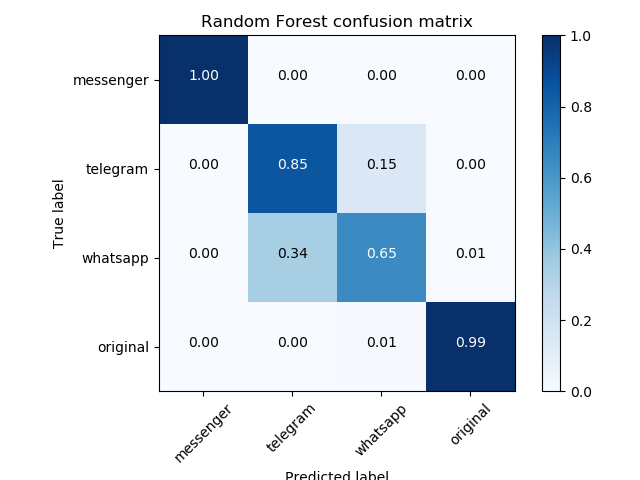
\includegraphics[scale=.6]{images/new_met_rf_initial_double_simple.png} 
\caption{random forest, last app classified} 
\end{figure} 


Result of the KFold validation with 10 bins:
 {\def\arraystretch{1.3} 
 \begin{table}[H] 
\centering 
\begin{tabular}{|l |l |l |l |l |l |l |l |l |l |}  
\hline 
0.8381&
0.8381&
0.8857&
0.9048&
0.8571&
0.8952&
0.8571&
0.8762&
0.8381&
0.8286\\ \hline  

\end{tabular} 
\end{table} }

The mean is : 0.861905